\documentclass[oneside,9pt]{memoir}

% Colors
\usepackage[dvipsnames]{xcolor}



% hyperref
\usepackage[%
    colorlinks=true,
    linktocpage=true,
    breaklinks=true,
    linkcolor=NavyBlue,
    urlcolor=NavyBlue,
    citecolor=NavyBlue
]{hyperref}
\def\chapterautorefname{§}
\def\sectionautorefname{§}
\def\subsectionautorefname{§}
\def\subsubsectionautorefname{§}

\setcounter{secnumdepth}{3}
\settocdepth{subsection}


% Fonts
\usepackage{fontspec}
\setmainfont[Numbers = {OldStyle, Proportional}]{TeX Gyre Pagella}
\setmonofont[Scale=MatchLowercase]{Menlo}

\usepackage{amsmath}
\DeclareMathOperator*{\argmax}{arg\,max}
\usepackage{unicode-math}
\setmathfont{TeX Gyre Pagella Math}

\usepackage{algorithm}
\usepackage[italicComments=false]{algpseudocodex}

\newcommand{\algorithmautorefname}{Algorithm}

% Typography
\usepackage[tracking]{microtype}

% Images
\usepackage{graphicx}

% ======================================================================
% Memoir package - layout and styling
% ======================================================================

% The calc package is required for calculating readable text widths
\usepackage{calc}

% Set outer and spine margins A wide right margin is chosen both for legibility
% of the typeblock and for tight integration of marginfigures and margin
% footnotes.

% Calculate widths in pts
\setlxvchars[\normalfont\normalsize] % about 66 characters per column
\setxlvchars[\normalfont\footnotesize] % about 45 characters per column

% Set left and right margins
\setlrmarginsandblock{1.15in}{3.5in}{*}
% Set upper and lower margins
\setulmarginsandblock{1.1in}{1.1in}{*}

% Set properties of margin notes, sidecaptioned floats, and footnotes in the
% margin.
\setmarginnotes{0.2in}{2.15in}{2\onelineskip}
\setsidecaps{0.2in}{2.15in}
\sidecapmargin{outer}
\renewcommand*{\sidecapstyle}{\normalfont\footnotesize}
\setsidecappos{c}


% Set footnotes in the margin rather than at the foot of the page
\footnotesinmargin
\setsidefeet{\marginparsep}{1.9in}{0.2in}{0pt}{\flushleftright\footnotesize}{*}

% Integrate the counters of the sidefootnotes and footnotes in margin.
\letcountercounter{sidefootnote}{footnote}
\setlength{\footmarkwidth}{0em}
\setlength{\footmarksep}{-\footmarkwidth}
\setlength{\footparindent}{1em}
\sideparmargin{outer}

\renewcommand*{\sideparfont}{\color{Maroon}\emphshape}
\renewcommand*{\sideparvshift}{2\baselineskip}
\marginparmargin{outer}

% Style the entries in the Table of Contents
\renewcommand*{\cftchapterfont}{\scshape\MakeTextLowercase}
\renewcommand*{\cftpartfont}{\color{Maroon}\scshape\MakeTextLowercase}
\captionstyle[\centering]{\footnotesize}
\captionnamefont{\footnotesize\color{Maroon}}

%% Bringhurst chapter and head styles with a Pedersen-type chapter number
\makechapterstyle{bringhurst}{%
	\renewcommand{\chapterheadstart}{} 
	\renewcommand{\printchaptername}{} 
	\renewcommand{\chapternamenum}{} 
	\setlength{\midchapskip}{15mm}
	\renewcommand*{\printchapternum}{%
        \begin{marginfigure}[0pt]
          \resizebox{!}{\midchapskip}{\color{Maroon}\emph{\thechapter}}
        \end{marginfigure}
      }
	\renewcommand{\afterchapternum}{} 
	\renewcommand{\printchaptertitle}[1]{%
	  \raggedright\Large\scshape\MakeLowercase{##1}}
	\renewcommand{\afterchaptertitle}{%
	  \vskip\onelineskip \hrule\vskip\onelineskip}
}
\setlength{\cftsubsectionindent}{0.6in}
\chapterstyle{bringhurst}
\headstyles{bringhurst}

\tightlists

% Headers and footers - page numbers, section headings, etc.
\makepagestyle{tufte}
\createmark{chapter}{left}{nonumber}{}{}
\makeoddhead{tufte}{}{}{\scshape\MakeTextLowercase{\leftmark}~~|~~\thepage}
\makeevenhead{tufte}{\thepage~~|~~\scshape\MakeTextLowercase{\rightmark}}{}{}
 \makerunningwidth{tufte}[8in]{8in}
\aliaspagestyle{chapter}{empty}
\nouppercaseheads
\pagestyle{tufte}

\linespread{1.1}
\checkandfixthelayout

% Bibliography management
\usepackage[%
    backend=biber,
    style=numeric-comp,
    sorting=none,
    natbib
]{biblatex}
\addbibresource{bibliography.bib}

\usepackage[backgroundcolor=white, bordercolor=white, textsize=small]{todonotes}

% =============
% Custom macros
% =============
\usepackage{textcomp}
\newcommand{\texthome}{\raisebox{0.5ex}{\texttildelow}}

\usepackage[cachedir=build, outputdir=build]{minted}

% ======================================================================
% Creating the title page
% ======================================================================

\title{SensorLab Seed Grant Report}
\author{\emph{Yuwei Wang, Vincent Raymond, Minh Duong, Adarsh Pyarelal}}
\begin{document}
\thispagestyle{empty}
\maketitle
\tableofcontents* 

\chapter{Summary}

In this report we describe the activities performed and milestones met for the
following SensorLab seed grants:

\begin{enumerate}
    \item Automated real-time detection of closed-loop communication in spoken
        dialogue.
    \item Development of an open-source dashboard for team communication
        experiments.
\end{enumerate}

The projects are complementary to each other, and targeted at enable studies of
real-time spoken team communication.

\chapter{Automated real-time detection of closed-loop communication in spoken dialogue}
\section{Task 1: Wearable audio streaming device (WASD)}

The goal of this task was to develop a wearable audio streaming device to
study spoken team dialog while bypassing the problem of audio source
separation.

Specifically, we wanted to write a program that would capture audio chunks on a
Raspberry Pi Zero 2 W device using a USB microphone, and stream the chunks to a
server over websockets. The chunks would then be fed to an automatic speech
recognition system to produce real-time transcriptions that could then be used
for further downstream analysis.

Unfortunately, while made a good deal of progress on this task, we were not
able to fully meet our proposed milestones. However, we did accomplish the
following:


\begin{itemize}
    \item \textbf{Hardware expertise development.} We were able to set up and get familiar with the Raspberry Pi
        devices, and setting up networking on Ubuntu in order to work with them
        wirelessly.

    \item \textbf{Software expertise development.} We developed general
        expertise in C and C++, and specific expertise in the mature libraries
        we chose for websockets (Boost.Beast) and audio recording (PortAudio).
        Notably, we learned to work with the quirks of using PortAudio on the
        Raspberry Pi.  We also developed a good understanding of writing
        programs to perform asynchronous I/O, which is necessary for performant
        audio streaming.

    \item \textbf{Dealing with audio on the Pi.} We also learned more on how to
        deal with audio recording on the Raspberry Pi, which turns out to be a
        non-trivial task due to the lack of documentation and the differences
        between the Linux distro on the Pi and the relatively heavier-weight
        Linux distros we are used to (e.g., Ubuntu).
        The undergraduate RA (Minh) developed a program to print all possible audio
        devices on the Pi, and at the same time, configure ALSA to choose the
        right default audio input device that is needed.

    \item \textbf{audioStreamer.} With the help of our research programmer
        (Vincent), we were able to develop an audio streaming program
        (\texttt{audioStreamer}) that can be started and stopped using control
        messages coming over an MQTT message bus. 

\end{itemize}

Some of the challenges we faced and lessons learned are listed below.

\begin{enumerate}

    \item \textbf{Hardware limitations} The Rasberry Pi took a fair amount of
        work to set up and interface with. This, coupled with its limited
        memory and processing power made it so that it was a non-trivial task
        to program on it (despite it being one of the more accessible
        single-board computers out there). 

        While we were able to get the
        \texttt{audioStreamer} program to compile fine on our laptop and
        desktop computers, the C++ libraries we used for the additional
        capabilities related to communicating with a message bus resulted in
        the compilation time on the Raspberry Pi being excessively long for
        regular development. We are exploring ways to mitigate this, such as
        precompiling non-audio hardware related code on a separate machine, and
        splitting up the code into smaller translation units to better leverage
        incremental compilation.

    \item Since we are dealing with a resource-limited device like the Pi, we
        chose to build our programs in C++ for efficient resource usage.
        However, C++ itself has a steep learning curve, as do the libraries we
        used (Boost.Beast for websockets and PortAudio for audio capture).
        While the undegraduate research assistant (Minh) on the project learned a lot
        from this task, the fact remains that the level of programming
        expertise required to perform this task within the proposed time frame
        is considerable.

        
\end{enumerate}


However, the work is not done, as the Pi is using a Linux distro with very
different setup and has very limited performance. Initially, when I tried to
build the program and run, Portaudio could not find the correct recording
device attached to the Pi. Thus I created a small Portaudio program that prints
out all possible audio devices on the Pi, and, at the same time, tried to
configure ALSA to make it choose the right default audio input device that I
need. Eventually, those changes made the program works on the Pi. However, the
program is stuck after running on the Pi for 1 - 2 seconds (which does not
occur on other Linux or Mac devices). After some changes to the program, I
found out that the problem occurs on the synchronous sending call to
Boost.Beast. Subsequently, the program needs to be edited so that it uses
Portaudio and Boost.Beast asynchronously.

After the first version of the program, Vincent also updated it to include more
features, namely the program can now listen to incoming messages and changes
its mode differently. However, these changes make the program quite large it
takes too long to build, and the Raspberry Pi does not have enough memory for
parallel compilation. Thus it is necessary to splitting up the program or to
compile it first on another machine and transfer it back to the Pi.

Current situation and objective

As of right now, although the program runs well on other machines, it cannot be
built on the Raspberry Pi because of its limited memory and processing power.
Thus the program needs to be split, or built on another machine and then
transferred back to the Pi. I am also currently setting up the ASR agent, which
is the endpoint that the audio is sent to, to test the AudioStreamer program.
After that, it is also necessary to test the working program on the Pi to check
if it runs properly without the problem of the previous version and to change
the Portaudio and Boost.Beast calls to become asynchronous.

\section{Task 2: Closed loop communication (CLC) detector}
\subsection{Introduction}

Closed-loop communication (CLC) is often recommended in the team research
literature as a communication behavior that can guarantee the accuracy of
information exchange. In this project, we developed a rule-based algorithm
based on event extraction from natural language for detecting the presence or
absence of CLC procedures in spoken dialogue within teams of humans
collaborating on shared tasks.

The ASR Agent in conjunction with the DialogAgent developed by the ToMCAT team
enables us to extract events of interest in real-time from spoken dialogue.
However, the DialogAgent works at the level of individual utterances, and does
not reason about multi-utterance context. 

\subsection{Approach}

There are three distinct phases in a complete Closed-loop communication:

\begin{enumerate}
    \item Call-out: The sender initiates a message.
    \item Check-back: The receiver acknowledges the message, usually by
        paraphrasing or repeating the main information of the message.
    \item Closed-loop: The sender verifies that the message has been received
        and interpreted correctly.
\end{enumerate}

Our rule-based EE system uses the Odin \cite{valenzuela-escarcega-etal-2016-odins}
event extraction framework, and currently contains 420 active rules that can
extract from simple to complex events, as well as entities and sentiment. Based
on these event rules, we develop an algorithm to detect the three phases of
CLC. First, the Call-out phase will be detected by rules in the DialogAgent.
Labels including HelpRequest, Instruction, and NeedAction are used as triggers
for this event. Next, we examine a window of the subsequent five utterances in
the dialogue.  If we find Move or Commitment labels by other team members as
well as the same semantic labels as in the Call-out message, then this
indicates there is a Check-back phase. However, we also care about the weak
Check-back situations where the team member only acknowledged the Call-out but
didn’t repeat the main information of the Call-out message. We assign the weak
version of Check-back a 0.5 score, compare to the full score of 1.  Finally,
within five utterances window, if we see the sender verified the information of
the Check-back with the Agreement label, we can determine that this is a
closed-loop communication. The final score of the Closed-loop communication
detected is the sum of the scores of the three phases.

\subsection{Evaluation}

To evaluate the algorithm of CLC detection, we conducted a CLC annotation task
for 3239 of the dialogue utterances from our ASIST Study-3 transcriptions, and
the rule-based CLC extractions and scores are tested on the golden annotation
regarding the precision, recall, and F1.


\subsection{Results}

Our CLC detection system extracted 978 closed-loop communication patterns,
scoring from 1.0, for which only the Call-out is detected but no Check-backs
and Closed-loop, to 4.0, for which two team members had checked back to one
call-out, and the initiator closed the loop at the end. However, our annotators
only detected 155 closed-loop communication patterns, indicating that the
rule-based CLC detection system is suffering from overgeneralizing issues at
this stage. A t-test between the CLC scores marked by the annotators and the
CLC scores assigned by our detection system shows that the CLC detection system
doesn’t give significantly higher scores for CLC detection than the annotators
(p > 1). 

\autoref{tab:clc} shows the results of our evaluation. Because the participants
in our game tasks are not specifically trained to use Closed-loop
communication, there is a relative rear distribution of the CLC pattern. We can
see from the table that although the overall F1 is as high as 0.79, the score
is largely boosted by the NA labels. Those are the utterances that don’t
recognize by the annotators and our system as a part of the closed-loop
communication.  However, for the individual phases of the CLC, we do see higher
recall scores than precision. This indicates that our rule-based CLC detection
system can pick as many of the phases as it can, but it also included too much
noise so that it’s not precise. 

\subsection{Error Analysis}

This result is caused by three major reasons: Firstly, for the Call-out phase,
there’s a competing nature between precision and recall. For example, the
Call-out is usually a question initiated by the initiator, but there are also a
fair amount of questions that don’t necessarily initiate a CLC session, like
``shall we go'', ``where are you''.  Secondly, when we look for recursive labels
between Call-out and potential Check-backs, overgeneralization could easily
happen to introduce noise. A lot of the time, the recursive labels are just
very common labels like Room or Victim, but the speakers are actually talking
about different things. Finally, the overmatching of the Close-loop phase is
generally caused by only looking for a simple acknowledgment or a Gratitude
label. But they are also very common labels that will easily cause
overmatching.



\begin{table}
    \centering
    \begin{tabular}{lrrrr}
        \toprule
                   & Precision & Recall & $F_1$ & Support\\\midrule
        NA         & 0.985     & 0.722  & 0.833 & 3084\\
        Call-out   & 0.123     & 0.774  & 0.212 & 155 \\
        Check-back & 0.118     & 0.721  & 0.203 & 147\\
        Close-loop & 0.021     & 0.550  & 0.041 & 20\\
        Overall    & 0.949     & 0.702  & 0.798 & 3239\\
        \bottomrule
    \end{tabular}
    \caption{Evaluation of the rule-based CLC detection system}
    \label{tab:clc}
\end{table}

\subsection{Conclusion}

As a creative method to break the limit of single utterances and building a
multi-speaker, multi-event extraction system in the context, this project made
an attempt to prove the potential of it. However, as the result is not ideal
for now, we see many areas that we should work on to adjust the current system.
For further development of the system, we’re also planning to introduce the
machine learning way to deal with the issues that rule-based system has issues
on. 

\chapter{Development of an open-source dashboard for team communication experiments}

The goal of this task was to create an open-source dashboard for controlling
and visualizing team communication experiments in real-time - i.e., to put a
more user-friendly interface on our existing backend infrastructure so that
other researchers at UArizona can utilize it more easily.

\section{Milestones}

We were able to partially complete Milestone 1 (real-time visualization of
automated transcriptions, dialog act classifications, and sentiment labels).
Specifically, we are able to now visualize automated transcriptions in
real-time (see \autoref{fig:asr_viz}).

\begin{figure}
    \centering
    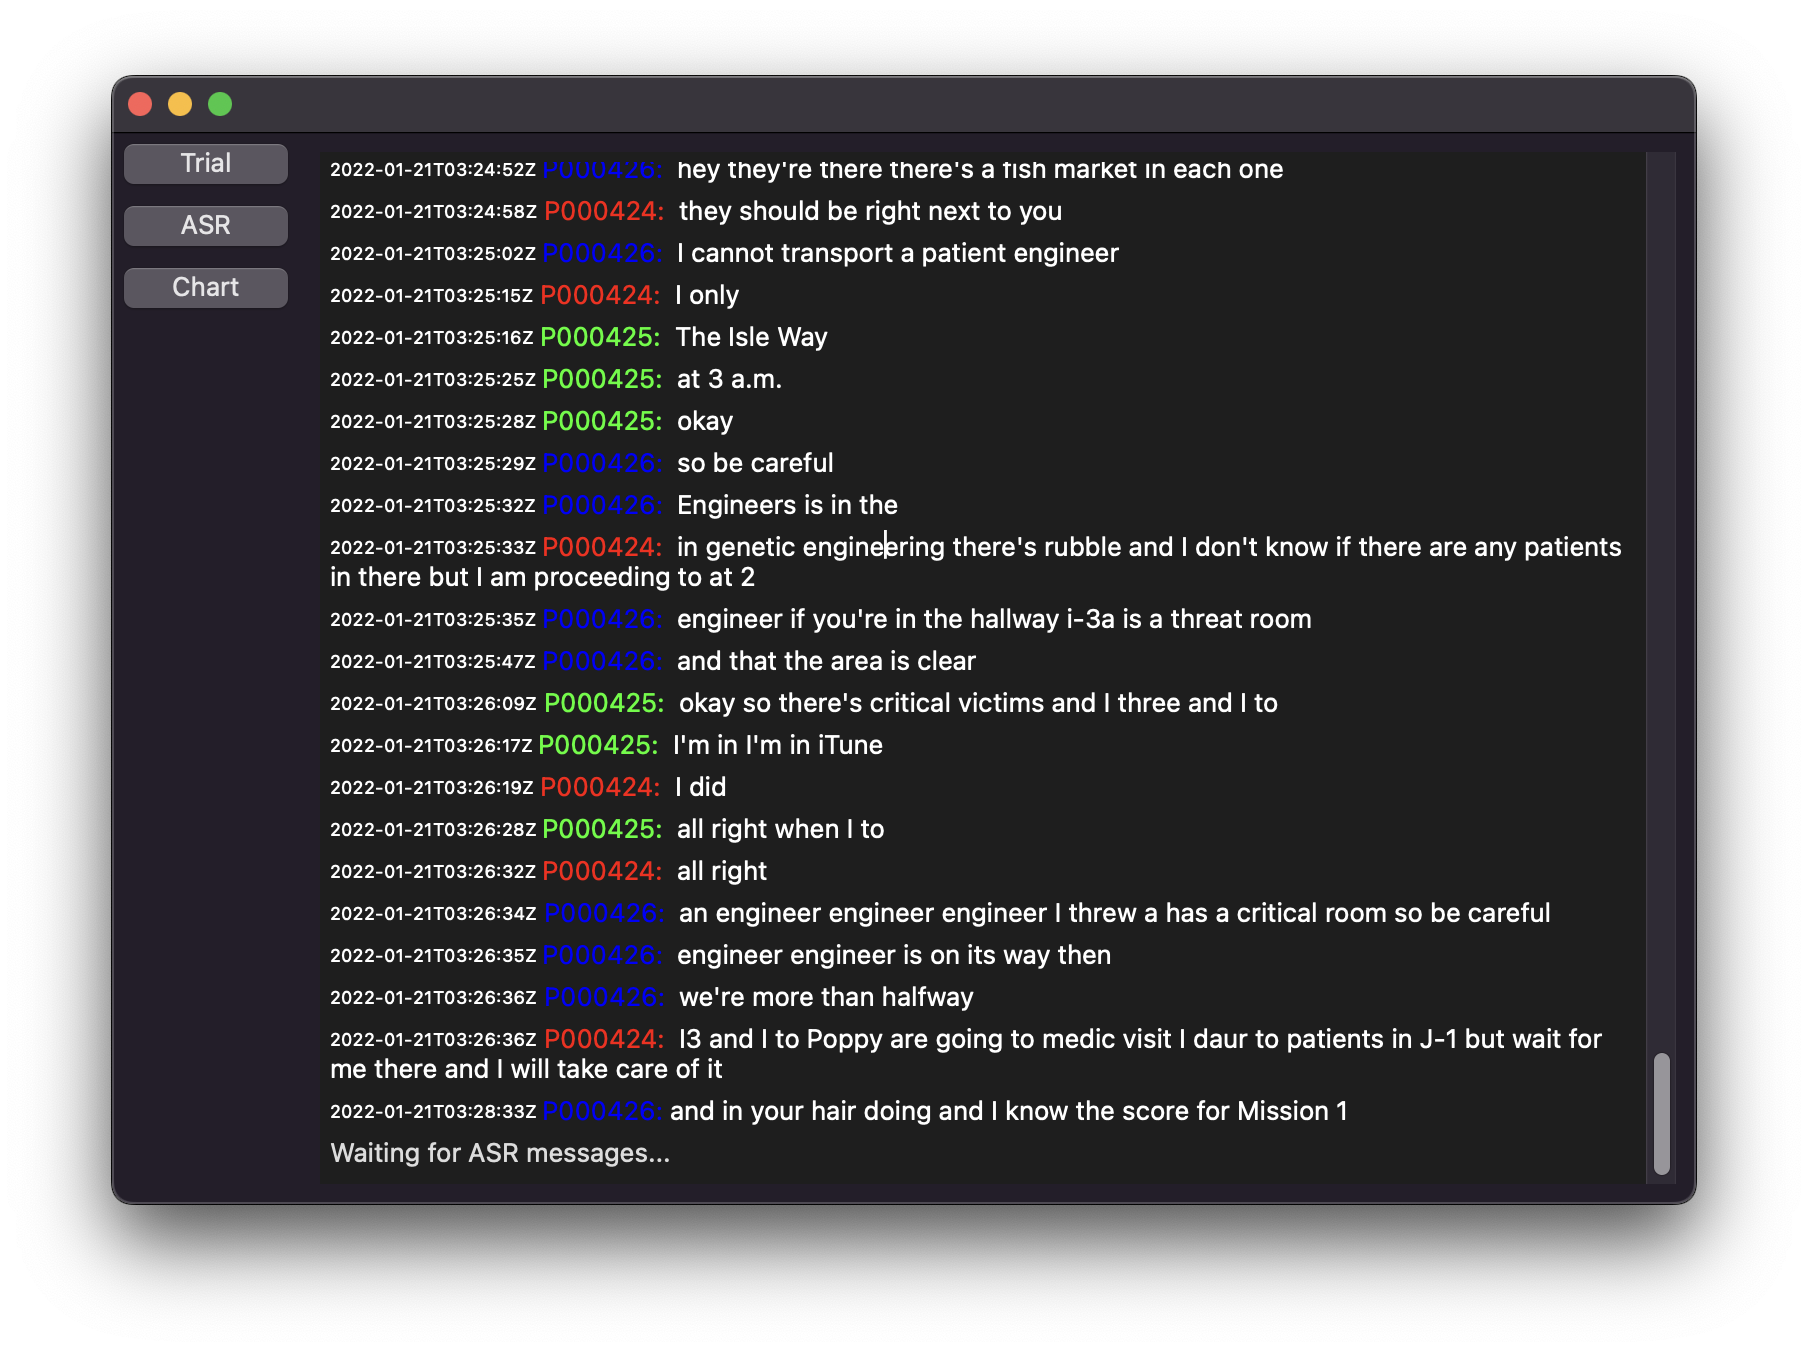
\includegraphics[width=\textwidth]{figures/asr_viz}
    \caption{ASR visualization during ongoing trial.}
    \label{fig:asr_viz}
\end{figure}

We did not implement visualization of dialog act classifications and sentiment
labels, but given our now-increased expertise in working with our visualization
libraries, we expect that it will not be too hard to implement those additions. 

We were not able to complete Milestone 2, since this milestone depended on the
development of the WASD sensors (\autoref{sec:wasd}), which we were not able to
complete on time.

In addition to these milestones, we implemented a generic interface for
real-time visualization of scalar values in dynamically updating charts.

\subsection{Prerequisites}

The following software components are required to build and run the dashboard.

\begin{enumerate}
    \item CMake: Build system for generating cross-platform Makefiles
    \item An MQTT message broker. We used Mosquitto for our testing.
    \item paho.mqtt.cpp: MQTT client library 
    \item nlohmann-json: Library for creating and parsing JSON messages
    \item wxWidgets: Cross-platform application and GUI development library
    \item Boost: Collection of miscellaneous C++ libraries.
\end{enumerate}

\subsubsection{macOS}

On macOS, if you are using the MacPorts package manager, you can install the
dependencies by invoking the following:

\begin{minted}{shell}
port install \
    cmake \
    mosquitto \
    paho.mqtt.cpp \
    nlohmann-json \
    wxWidgets-3.2 \
    boost
\end{minted}

You will also need to activate \texttt{wxWidgets-3.2} by running:

\begin{minted}{shell}
port select --set wxWidgets wxWidgets-3.2
\end{minted}

\subsubsection{Ubuntu}

Similarly, from Ubuntu 21.10 onwards, all dependencies can be installed through
the \texttt{apt} package manager.

\begin{minted}{shell}
apt install \
        cmake \
        mosquitto \
        libpaho-mqtt-dev \
        libpaho-mqttpp-dev \
        libssl-dev \
        nlohmann-json3-dev \
        libboost-all-dev \
        libwxgtk3.0-gtk3-dev
\end{minted}

Note: The \texttt{paho.mqtt.cpp} library  is not available through \texttt{apt}
prior to Ubuntu 21.10. If using an earlier version of Ubuntu, the library will
need to be installed from source.

\subsection{Building}

The ToMCAT Dashboard uses CMake to generate cross-platform Makefiles. This
makes it easy to build the program once all dependencies are installed. After
cloning the repository, to build the dashboard, run the following from the root
directory.

\begin{minted}{shell}
mkdir -p build
cd build
cmake ..
make -j
\end{minted}


\subsection{Running the dashboard}

\subsubsection{Launch MQTT broker}

The ToMCAT Dashboard connects to an MQTT message bus for processing incoming
data and communication between components. Before running the dashboard, an
MQTT broker must be launched, if one is not already running.  You may need to
prefix the invocations below with \mintinline{shell}{sudo}.

\begin{itemize}
    \item If you have MacOS with MacPorts: \mintinline{shell}{port load mosquitto}
    \item Ubuntu: \mintinline{shell}{service mosquitto start}
\end{itemize}

\subsubsection{Configure MQTT broker}

By default, the dashboard will attempt to connect to an MQTT broker running on
port 1883 of localhost. This can be configured in the \texttt{config/app.json} file by
modifying the following values:

\begin{itemize}

    \item \texttt{mqtt\_host}: (default=0.0.0.0) The host that the MQTT broker
        is running on.

    \item \texttt{mqtt\_port}: (default=1883) The port that the MQTT broker is
        running on.

\end{itemize}

\subsubsection{Run dashboard}

\begin{minted}{shell}
./gui
\end{minted}



\subsection{Visualization}

\subsubsection{ASR}

Example ASR Message:

\begin{minted}{JSON}
{
  "data": {
    "text": "I am going to save a green victim.",
    "is_final": true,
    "id": "59678a5f-9c5b-451f-8506-04bc020f2cf3",
    "participant_id": "participant_1",
    "start_timestamp": "2021-01-19T23:27:57.978016Z",
    "end_timestamp" : "2021-01-19T23:27:58.633076Z"
   },
  "header": {
    "timestamp": "2021-01-19T23:27:58.633076Z",
    "message_type": "observation",
    "version": "0.1"
  },
  "msg": {
    "timestamp": "2021-01-19T23:27:58.633967Z",
    "experiment_id": "e2a3cb96-5f2f-11eb-8971-18810ee8274e",
    "trial_id": "256d1b4a-d81d-465d-8ef0-2162ff96e204",
    "version": "3.3.2",
    "source": "speech_analyzer_agent",
    "sub_type": "asr:transcription"
  }
}
\end{minted}


Usage

To visualize incoming ASR utterances, navigate to the ``ASR" tab in the menu
sidebar. At the start of the trial, the panel on the right will display the text
``Waiting for ASR messages…''.

Image 1: ASR visualization at trial start

As the trial progresses, and ASR messages come in, they will fill the panel one
line at a time. In addition to the utterance text itself, each line will also
contain a timestamp of when the utterance was generated, and a participant id
colored to match the associated color of the participant.

Image 2: ASR visualization during ongoing trial

This color can be Red, Blue, or Green, and the mapping between color and participant comes from the Trial Start message.

Charting
Chart Configuration
The data being charted can be configured by modifying the ``ChartWidget” section in conifg/conf.json.

\begin{minted}{JSON}
"ChartWidget":{
                 "topics":[
                        "score"
                ],
                "x_axis_field": "Time",
                "x_axis_label": "Time",
                "y_axis_field": "Score",
                "y_axis_label": "Score",
                "panel_name": "CHART_PANEL"
 }
\end{minted}

The dashboard will listen for incoming messages on any topics listed in the
``topics” field. When processing messages, it will then check for the fields
defined by ``x\_axis\_field'' and ``y\_axis\_field”, create an x/y point, and
add that point to the chart. ``x\_axis\_label'' and ``y\_axis\_label'' are used to
add a label to the x-axis and y-axis of the chart. Finally, ``panel\_name'' is
used internally by the dashboard, and should not be modified.  Example Chart
Message

\begin{minted}{JSON}
{
        "data":{
                "Time": 0.2,
                "Score": 10
        }
}
\end{minted}



Note:
1. The ``Time” and ``Score” fields are not at the root level of the JSON message, but a part of the ``data” field. This is to keep the formatting consistent with for other message types used by the dashboard.
2. Each message should contain exactly one x/y pair. Other fields can be included, but will be ignored
3. Data points should be either an integer or float value

Usage
To visualize data being charted, navigate to the ``Chart” tab in the menu sidebar. At the start of the trial, the right-side panel will display an empty graph. If a label for the x-axis or y-axis was defined in the configuration, those labels will be displayed on the axes.  By default, the graph will be centered around point (0,0)
Image 3: Chart visualization before trial start

When adding a data point, if the data point is outside the visible range, the chart will automatically fit the data and adjust the x-axis and y-axis so that the new data point can be seen.


Image 4: Chart visualization during ongoing trial


\printbibliography
\end{document}
